\documentclass[10pt,twocolumn,letterpaper]{article}

\usepackage{cvpr}
\usepackage{times}
\usepackage{epsfig}
\usepackage{graphicx}
\usepackage{amsmath}
\usepackage{amssymb}

% Include other packages here, before hyperref.

% If you comment hyperref and then uncomment it, you should delete
% egpaper.aux before re-running latex.  (Or just hit 'q' on the first latex
% run, let it finish, and you should be clear).
\usepackage[breaklinks=true,bookmarks=false]{hyperref}

\cvprfinalcopy % *** Uncomment this line for the final submission

\def\cvprPaperID{****} % *** Enter the CVPR Paper ID here
\def\httilde{\mbox{\tt\raisebox{-.5ex}{\symbol{126}}}}

% Pages are numbered in submission mode, and unnumbered in camera-ready
%\ifcvprfinal\pagestyle{empty}\fi
\setcounter{page}{4321}
\begin{document}

%%%%%%%%% TITLE
\title{Fully Convolutional Networks for Image Segmentation with keras}

\author{Giacomo Barzon\\
{\tt\small giacomo.barzon.2@studenti.unipd.it}
% For a paper whose authors are all at the same institution,
% omit the following lines up until the closing ``}''.
% Additional authors and addresses can be added with ``\and'',
% just like the second author.
% To save space, use either the email address or home page, not both
\and
Giacomo Greggio\\
{\tt\small giacomo.greggio.1@studenti.unipd.it}
\and
Diego Mazzalovo\\
{\tt\small diego.mazzalovo@studenti.unipd.it}
}
\maketitle
%\thispagestyle{empty}

%%%%%%%%% ABSTRACT
\begin{abstract}
	"Fully Convolutional Networks for Semantic Segmentation"\cite{projectPaper} is one of the most important piece of work related to Image Semantic Segmentation. Our aim is to reproduce the architectures proposed by the authors which are based on Fully Convolutional Networks (FCNs) with skip connections.
	We trained and tested these architectures on the PASCAL VOC 2011 dataset and we obtain a meanIU of TODO. In addition, we trained and tested the architectures on other datasets as the carvana-image-masking. Since the dataset is much simpler than the previous, the results that we obtained are better than the results on PASCAL VOC 2011, and we reach a meanIU of TODO.
\end{abstract}

%%%%%%%%% BODY TEXT
\section{Introduction}

When we talk about Image data there are many tasks that can come to mind. The easiest one that someone can implement is image classification: you give as input an image to the suitable classifier and this one returns the label related to the object that it represents. \\
This approach to image classification has some serious limits, for example if your image contains various objects belonging to several different classes, it's basically impossible to find the correct label since multiple labels will be associated to that image. Moreover in many applications knowing the content of an image is not enough, and it comes necessary to find the locations of the objects depicted in it. \\
The next step to naive image classification is object detection. In object detection, we not only need to identify all the objects of interest in the image, but also their positions. The positions are generally represented by a rectangular bounding box. \\
This approach can be improved because the boxes don't identify perfectly the object boundaries. In many fields like autonomous driving or medical applications knowing the exact boundaries is essential.
So, the next step that can be made to improve object detection is image segmentation.
Image segmentation, is the task of clustering parts of an image together which belong to the same object class. The predictions are made over each pixel which is classified according to a category which can be background or the class it is associated to. \\
There are many more tasks related to image data, but we will focus only on image segmentation. \\ \\
Image classification task are often handled by convolutional networks that have fully connected dense layers at the end of the network. This approach may be fine for many different applications but can pose some serious limitations for image segmentation. The main one is that dense layers unlike convolutional ones can't handle images of various size. To solve this problems many different approaches have been proposed like resizing the images or patch sampling, that we discuss better in the next section. \\ \\
All of these methods though can handle only fixed input size or require complicated preprocessing and machinery in order to work. In fully convolutional networks (FCNs) dense layers are substituted by convolutional ones, to make them capable to manage images of any size and produce an output of the same size of the image. TO DO


\section{Related Work}

There are many different approaches to solve semantic segmentation problems. The most common approach inolve ConvNets with dense predictions. Since they can't handle input of different sizes, many different processing techniques had to be taken in order to make segmentation work. For example, by sampling an area of fixed dimension around each pixel and  using that to classifying the pixel. Some previous works have been done by Ning et al.\cite{1495508}, Cirean et al.\cite{article}, where they applied image segmentation respectively to the evolution of embryos and to neuroanatomy. \\
This method computes a prediction pixel by pixel, so both training and predicting, are computationally not efficient. \\ \\
As time passed better approaches have been developed like FCNs that we will discuss in the other chapters, but also many other different techniques.\\
For example one of the most popular way (from what we have seen) to solve semantic segmentation is through the use of encoder-decoder architectures (see fig. \ref{ednet}).
\begin{figure}[t]
	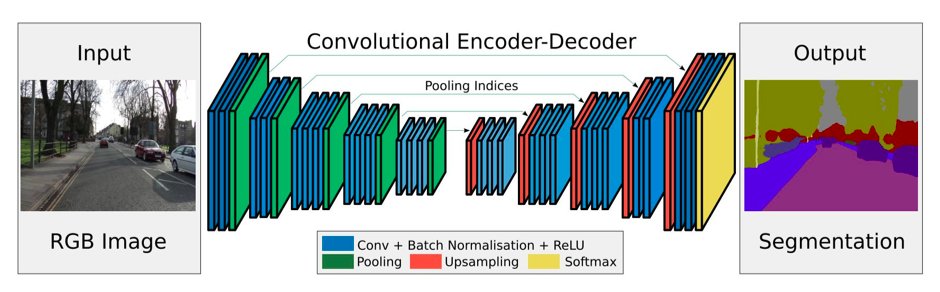
\includegraphics[width=8cm]{image/ednet}
	\label{ednet}
	\centering
	\caption{Encoder-decoder architecure}
\end{figure}
The encoder-decoder architecures are made by two parts: an encoder using convolutional layers (usually taken by VGG16) and deconvolutional network which takes in input the feature vector produced by the encoder and generates a map of pixelwise class probabilities. Some works have been made by Li et al.\cite{8379359} and Weng et al.\cite{8681706}.\\ \\
Many different approaches based on recursive and recurrent neaural networks have also been proposed, but we didn't dive to much on that. For a more detailed description of the state of the art check the survey made by Minaee et al.\cite{unknown}. 


\section{Dataset}

Since our goal is to reproduce one or more experiments made by the reference paper\cite{projectPaper}, we chose to use the PASCAL VOC 2011\cite{pascal-voc-2011} dataset in which the authors tested all their architectures.
The dataset refers to a visual object challenge made in 2011 and which has been updated in the next years. \\
The dataset contains more than 10000 images with annotations related to different tasks like classification, object detection and image segmentation.
For our task it contains 2223 images, which are 1112 for training set and 1111 for validation set.
The segmentation data is composed by 21 different classes, including background, and a void label which is used to identify the pixels that are ambiguous or difficult to classify, these pixel should be ignored when calculating the loss value.
As validation data we used a subset of 736 images like it was done in \cite{projectPaper}, according to "Semantic Boundaries Dataset and Benchmark"\cite{BharathICCV2011}. \\ \\
Before testing on PASCAL VOC 2011 dataset, we tested also in a simpler dataset: "Carvana-image-masking-challenge"\cite{carvana} dataset. This dataset was published by Carvana for a challenge on Kaggle. It contains over 5000 images of different kind of cars seen from various angles. Segmentation data contains only 2 classes: the background and the cars' one. \\
The training on Carvana's dataset took less time and epochs to converge to nice results. TO DO
This was mainly due to the fact that all images contained in the dataset shared the same background. Also the more limited amount of classes that the network needed to predict, helped a lot to speed up the convergence. TO DO \\ \\
All the segmentation datasets contain two main components: the image data and the mask data. Image data do not require more explanations. Mask data are the classification targets, they have the same shape of the images related to them and each pixel in the mask represent the class it belongs to.
Basically all the datasets needed a minimum amount of preprocessing.
Since all the mask are in RGB format and the neural network returns a probability distribution over each class, we needed to convert the three channels to a single channel representing in each entry the corresponding class. Initially we converted each image to a one-hot-encoding where the number of channels was equal to the number of classes. After some experiments we found out that this wasn't necessary, so we decided to use a lighter version with only one channel. \\
In addition to that, we also normalized the images, in order to obtain only values between 0 and 1. This is important to avoid gradient explosion issues, but it isn't a mandatory step to train the network.
Since we couldn't load the entire dataset in the memories of our PCs, we were forced to build a data generator. A data generator is an object which can be called by keras and returns only the data required to execute a single batch step. This allows us to keep in memory much less data.

\section{Method}

The authors of \cite{projectPaper} wrote all of their implementations using Caffe \footnote{\href{https://caffe.berkeleyvision.org/}{Link to Caffe}}, a public library with many tools suitable for computer vision. On the other hand we used for all our implementations Keras \footnote{\href{https://keras.io/}{Link to Keras}} library. \\
One of the first things we did was reproducing the architectures that were illustrated in the paper. The most basic architecture between the ones that we reproduced is the FCN32. This architecture is made starting from the VGG16 architecture \cite{weights}.
\begin{figure}[t]
	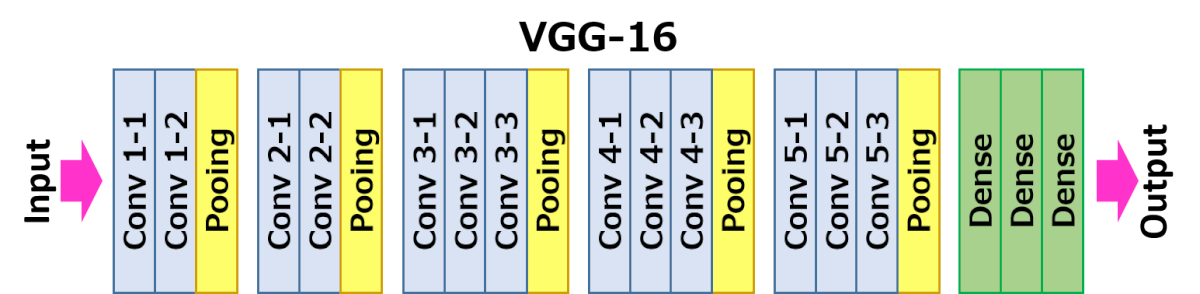
\includegraphics[width=8cm]{image/vgg16}
	\label{vgg}
	\centering
	\caption{VGG16 architecure}
\end{figure}
Like we can see in \ref{vgg} the VGG16 architecture is made by five convolutional blocks, each one contains two or three convolutional layers followed by a MaxPooling layer. After those convolutional blocks there are three fully connected dense layers, which are responsible to make predictions.
\subsection{FCN-32}
We started by replicating the whole VGG16 network with basic keras layers. Since we needed the network to handle inputs of various sizes, we removed the last three fully connected dense layers of the VGG16. Then, we downloaded the pretrained weights of the remaining layers of the network available in the public library of keras.
Like the authors of \cite{projectPaper} did, we appended at the end of the networks three convolutional layers. The first one has a number of filters of 4096 and a kernel size of (7x7). The second one also has a number of filters of 4096, but a kernel size of (1x1). The last one has a number of filters equal to the number of classes we want to predict and a kernel size of (1x1).
These last three layers act in substitution of the dense layers that we removed from the original VGG16. They are the ones who make predictions, but since they are convolutional, they can still handle inputs of any size.
Moreover between each one of these last three convolutional layers we also put a dropout layer with p=0.5.\\
As of now the network outputs a tensor which has a size significantly lower than the one of the input image. Since we want the output to have the same size of the input, we needed to add a deconvolutional layer of size (64x64) with stride 32. This layer increases the size of the input it receives by applying a deconvolution operation. In keras this layer takes the name of Conv2DTranspose \footnote{\href{https://www.tensorflow.org/api_docs/python/tf/keras/layers/Conv2DTranspose}{Link to Conv2DTranspose}}. However, this operation made the output of the network too big by a few extra pixels.\\
\begin{figure*}
	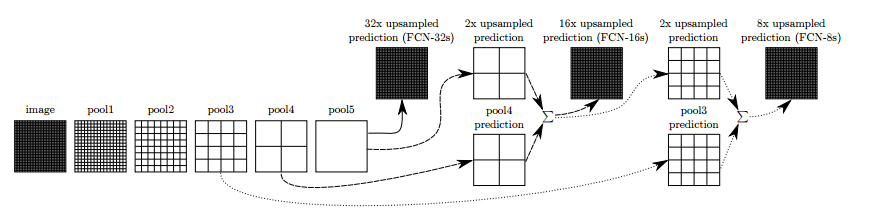
\includegraphics[width=\textwidth]{image/fcn}
	\label{fcn}
	\centering
	\caption{FCN architecure}
\end{figure*}
To solve the problem the authors of the paper added a Cropping layer which takes in input the outputs of two layers and resizes the biggest one to the dimension of the smaller one by removing the extra pixels from the borders. Keras does not implement dynamic cropping, so we needed to implement a custom layer to perform the dynamic crop operation. At the end of the network there is a softmax layer in order to produce a valid probability distribution over each class.
\subsection{FCN-16}
This architecture is fine, but it can be improved. A way to improve performances is by implementing skip architectures. The receptive fields of the deeper layers are bigger and see more pixels if compared with the shallower ones. This causes FCN32 to produce coarse outputs. Combining the outputs of the deeper layers with the outputs of the shallower ones, allows the model to make more local predictions while respecting the global structure. \\
FCN16 is built on this idea. We take the output of the fourth convolutional block of FCN32 and apply a convolution to it with kernel size of (1x1) and number of filters equal to the number of classes that we want to predict. Then, we sum it with the last convolutional layer of FCN32, the one immediately before the deconvolutional layer. We call this operation fusion  as the original paper. The dimension of the obtained convolutional layer is bigger than the one of the last convolutional layer, due to an higher amount of pooling operations applied to this last layer. 
To make the dimensions of their outputs match we apply to the smaller one a deconvolution with number of filters equal to the number of classes, kernel size of (1x1) and stride equal to 2. We crop the extra pixels with our custom cropping layer like we did at the end of FCN32. Then to make the dimensions of the output match the input dimensions we applied another time a deconvolution followed by a crop.
\subsection{FCN-8}
FCN16 improves a lot the results of FCN32, but it can still be improved. To do that, we follow the same process we used to build FCN16 with some small differences and obtain FCN8.
We take the output of the third convolutional block of VGG16 and apply a convolution to it with the same parameters as the previous architecture and fuse it with the fusion layer of FCN16. As we have done with FCN16 we applied a deconvolution with kernel size of (4x4), stride equal to 2 and number of classes filters. We need to crop the biggest one between the two before fusing them together. As last layer we make the convolution of the fusion layer with number of classes filters and kernel size of (16x16) and stride equal to 8 which we have to crop to obtain the same dimensions as the input image. The last layer is a softmax layer to produce a valid probability distribution over each class. \\
On all convolutional layers we applied padding in order to obtain the same dimension of the input images. Moreover, all convolutional layers had ReLU as activation function, while the others had a linear activation function. \\ \\
Like the authors of \cite{projectPaper} we didn't bother fusing even shallowers layers, since also between FCN-16 and FCN-8 there was a small improvement (TO DO)


\section{Experiments}

\section{Conclusions}

\subsection{Suggested Structure}

The following is a suggested structure for your report:

\begin{itemize}
	\item Introduction (10\%): describe the problem you are working on, why it's important, and an overview of your results.
	\item Related Work (10\%): discuss published work or similar apps that relates to your project. How is your approach similar or different from others? 

	\item Dataset (15\%): describe the data you are working with for your project. What type of data is it? Where did it come from? How much data are you working with? Did you have to do any preprocessing, filtering, etc., and why?
	\item Method (30\%): discuss your approach for solving the problems that you set up in the introduction. Why is your approach the right thing to do? Did you consider alternative approaches? It may be helpful to include figures, diagrams, or tables to describe your method or compare it with others.
	\item Experiments (30\%): discuss the experiments that you performed. The exact experiments will vary depending on the project, but you might compare with prior work, perform an ablation study to determine the impact of various components of your system, experiment with different hyperparameters or architectural choices. You should include graphs, tables, or other figures to illustrate your experimental results.
	\item Conclusion (5\%): summarize your key results; what have you learned? Suggest ideas for future extensions.
\end{itemize}	

%------------------------------------------------------------------------
\section{Formatting your paper}

All text must be in a two-column format. The total allowable width of the
text area is $6\frac78$ inches (17.5 cm) wide by $8\frac78$ inches (22.54
cm) high. Columns are to be $3\frac14$ inches (8.25 cm) wide, with a
$\frac{5}{16}$ inch (0.8 cm) space between them. The main title (on the
first page) should begin 1.0 inch (2.54 cm) from the top edge of the
page. The second and following pages should begin 1.0 inch (2.54 cm) from
the top edge. On all pages, the bottom margin should be 1-1/8 inches (2.86
cm) from the bottom edge of the page for $8.5 \times 11$-inch paper; for A4
paper, approximately 1-5/8 inches (4.13 cm) from the bottom edge of the
page.

%-------------------------------------------------------------------------
\subsection{Margins and page numbering}

All printed material, including text, illustrations, and charts, must be kept
within a print area 6-7/8 inches (17.5 cm) wide by 8-7/8 inches (22.54 cm)
high.
Page numbers should be in footer with page numbers, centered and .75
inches from the bottom of the page and make it start at the correct page
number rather than the 4321 in the example.  To do this fine the line (around
line 23)
\begin{verbatim}
%\ifcvprfinal\pagestyle{empty}\fi
\setcounter{page}{4321}
\end{verbatim}
where the number 4321 is your assigned starting page.

Make sure the first page is numbered by commenting out the first page being
empty on line 46
\begin{verbatim}
%\thispagestyle{empty}
\end{verbatim}


%-------------------------------------------------------------------------
\subsection{Type-style and fonts}

Wherever Times is specified, Times Roman may also be used. If neither is
available on your word processor, please use the font closest in
appearance to Times to which you have access.

MAIN TITLE. Center the title 1-3/8 inches (3.49 cm) from the top edge of
the first page. The title should be in Times 14-point, boldface type.
Capitalize the first letter of nouns, pronouns, verbs, adjectives, and
adverbs; do not capitalize articles, coordinate conjunctions, or
prepositions (unless the title begins with such a word). Leave two blank
lines after the title.

AUTHOR NAME(s) and AFFILIATION(s) are to be centered beneath the title
and printed in Times 12-point, non-boldface type. This information is to
be followed by two blank lines.

The ABSTRACT and MAIN TEXT are to be in a two-column format.

MAIN TEXT. Type main text in 10-point Times, single-spaced. Do NOT use
double-spacing. All paragraphs should be indented 1 pica (approx. 1/6
inch or 0.422 cm). Make sure your text is fully justified---that is,
flush left and flush right. Please do not place any additional blank
lines between paragraphs.

Figure and table captions should be 9-point Roman type as in
Table~\ref{mytable}. Short captions should be centred.

\noindent Callouts should be 9-point Helvetica, non-boldface type.
Initially capitalize only the first word of section titles and first-,
second-, and third-order headings.

FIRST-ORDER HEADINGS. (For example, {\large \bf 1. Introduction})
should be Times 12-point boldface, initially capitalized, flush left,
with one blank line before, and one blank line after.

SECOND-ORDER HEADINGS. (For example, { \bf 1.1. Database elements})
should be Times 11-point boldface, initially capitalized, flush left,
with one blank line before, and one after. If you require a third-order
heading (we discourage it), use 10-point Times, boldface, initially
capitalized, flush left, preceded by one blank line, followed by a period
and your text on the same line.

%-------------------------------------------------------------------------
\subsection{Footnotes}

Please use footnotes\footnote {This is what a footnote looks like.  It
often distracts the reader from the main flow of the argument.} sparingly.
Indeed, try to avoid footnotes altogether and include necessary peripheral
observations in
the text (within parentheses, if you prefer, as in this sentence).  If you
wish to use a footnote, place it at the bottom of the column on the page on
which it is referenced. Use Times 8-point type, single-spaced.


%-------------------------------------------------------------------------
\subsection{References}

List and number all bibliographical references in 9-point Times,
single-spaced, at the end of your paper. When referenced in the text,
enclose the citation number in square brackets, for
example~\cite{Authors14}.  Where appropriate, include the name(s) of
editors of referenced books.

\begin{table}
\begin{center}
\begin{tabular}{|l|c|}
\hline
Method & Frobnability \\
\hline\hline
Theirs & Frumpy \\
Yours & Frobbly \\
Ours & Makes one's heart Frob\\
\hline
\end{tabular}
\end{center}
\caption{Results. Ours is better.}
\label{mytable}
\end{table}

%-------------------------------------------------------------------------
\subsection{Illustrations, graphs, and photographs}

All graphics should be centered.  Please ensure that any point you wish to
make is resolvable in a printed copy of the paper.  Resize fonts in figures
to match the font in the body text, and choose line widths which render
effectively in print.  Many readers (and reviewers), even of an electronic
copy, will choose to print your paper in order to read it.  You cannot
insist that they do otherwise, and therefore must not assume that they can
zoom in to see tiny details on a graphic.

When placing figures in \LaTeX, it's almost always best to use
\verb+\includegraphics+, and to specify the  figure width as a multiple of
the line width as in the example below
{\small\begin{verbatim}
   \usepackage[dvips]{graphicx} ...
   \includegraphics[width=0.8\linewidth]
                   {myfile.eps}
\end{verbatim}
}


{\small
\bibliographystyle{ieee_fullname}
\bibliography{egbib}
}

\end{document}
